%
% File: chap03-02-01.tex
% Author:
% Description:
% 3.2 Front-end Design & Implementation
%  3.2.1 Early Stage-Virtual Hospital Africa(VHA)
%
%

\paragraph{Design Process}\mbox{}\\
During initial discussions with the client about their requirements, the client pointed out that the current website's Patient Intake page contained too many information fields, leading to poor user experience and even many testers abandoning the form midway during testing (Figure 3.1). Based on this situation, the client designed a second version of the multi-step form interface (Figure 3.2). The original form was split into separate pages (personal information, contact information, primary care, reason for visit), each with a progress indicator to guide users through the process.

During the programming and testing of the second version design, group members identified several issues that could potentially impact usability in actual interactions. We conducted internal team discussions and shared these issues with the client during our weekly design meetings. Ultimately, the client adopted our suggestions and finalized the third version design (Figure 3.3), with the following key improvements:

\begin{itemize}
    \item 1. Added a left-side navigation bar to enable non-linear navigation
\end{itemize}
The original design relied solely on the top progress bar, requiring users to complete steps in a fixed order. We suggested adding a modular navigation bar on the left side, allowing users to freely jump to any section for modifications, thereby enhancing their sense of control and flexibility \cite{nielsen1995}.

\begin{itemize}
    \item 2. Optimized field grouping and information hierarchy
\end{itemize}
We consolidated information such as name, gender, title, language, and national ID number into the “General” group and introduced a profile photo upload function on this page to add a patient profile photo capture/upload feature. This aligns the website's information layout with users' real-world information collection habits and aligns with the standard practice in hospital admission processes of “first collecting basic information and taking photos for record-keeping.” Additionally, once the avatar upload is complete, a preview will be displayed immediately, and the centralized presentation of related fields will allow users to quickly confirm the accuracy of key information in a unified area, ensuring visibility of the interaction process \cite{nielsen1995}.

\begin{itemize}
    \item 3. Unify navigation button layout
\end{itemize}
In the third version design, since we removed the top global navigation bar, users need clearer prompts for the next steps in the interface. Based on Nielsen's (1995) usability principles of “Visibility of system status” and “Match between system and the real world,” we replaced the bottom buttons with ‘Back’ and “Next” as alternative navigation methods, clearly indicating the user's forward and return paths. This design reduces users' sense of disorientation during task flows, enhances the predictability of operations, and increases the certainty of task completion.

Regarding the second group: The client's requirements primarily focused on the patient profile page, highlighting several shortcomings in the current interface regarding information presentation and user experience. These include lack of detailed patient identification methods and information, absence of quick access points, unclear information structure, absence of direct editing functions, low efficiency in switching between information modules, and insufficient visual hierarchy in the interface (Figure 3.4). In response to the client's requirements, we proposed several improvement suggestions, which were confirmed in subsequent meetings with the client, ultimately resulting in the design of the new version (Figure 3.5):

\begin{itemize}
    \item 1. Enhance the patient information card: Add a profile picture, gender/age tags, patient status, quick contact button, download patient report button, and last edit time to the patient information card. This not only avoids healthcare staff having to make additional clicks or page switches to confirm patient identity and status but also addresses the issue of being unable to perform common operations directly on the patient profile page, enabling quick identification and efficient management of patient information.
    \item 2. Expand the patient information module and optimize the information navigation structure: Introduce more patient information modules in the Patient Profile, unify the naming and order of the top tab bar, and add a secondary menu on the left side, dividing the information into modules such as General, Primary Care, Contacts, Biometrics, and Insurance. This modular structure enhances the completeness of the information, allowing users to efficiently obtain the required data on a single page and reducing the need for frequent page switching or scrolling to find information.
    \item 3. Switch to editable forms: Present personal information in structured fields that support direct editing. This simplifies the information maintenance process, reduces operational steps, and enhances the user experience.
\end{itemize}
The third group of customers' needs were mainly focused on the Vitals page, and they pointed out that the current interface had many shortcomings in terms of data input structure and interaction experience, mainly including: all vital signs items were stacked in a single list, with no clear distinction between required and optional fields, making it difficult for users to quickly identify which fields to fill in first; the order of the fields did not fully match the clinical data collection process, and some commonly used data items were not placed prominently enough; the page lacked step-by-step navigation or process guidance, and users might not be able to confirm their progress(Figure 3.6). After internal discussions, we proposed improvement suggestions for these issues and reached consensus with the client during meetings, ultimately finalizing the new version design (Figure 3.7):

\begin{itemize}
    \item 1. Grouped layout and priority adjustments
\end{itemize}
Vital sign information is divided into two main sections: “Required” and “Optional,” ensuring that healthcare professionals prioritize the collection of critical data; the field order is adjusted to better align with actual clinical data collection practices (e.g., first entering height, weight, temperature, blood pressure, and pulse rate, followed by optional items such as blood glucose, oxygen saturation, and respiratory rate) \cite{webform}.

\begin{itemize}
    \item 2. Optimized operational workflow
\end{itemize}
Added Back/Next navigation buttons at the bottom of the page to replace the original single “Continue” button, allowing users to more intuitively control the progress of form completion and avoid omissions due to skipping or accidental operations.

\begin{itemize}
    \item 3. Integration with patient information panel
\end{itemize}
Retained the patient profile summary and treatment timeline (Seeking Treatment) on the right side, ensuring that healthcare professionals can reference the patient's status and completed examination steps at any time during data entry.

These changes adhere to usability principles such as “Match between system and the real world,” “Visibility of system status,” and “Recognition rather than recall,” reducing cognitive load, improving data entry efficiency, and minimizing operational errors \cite{nielsen1995}.

\begin{figure}[H]
    \centering
    \begin{minipage}{0.47\textwidth}
        \centering
        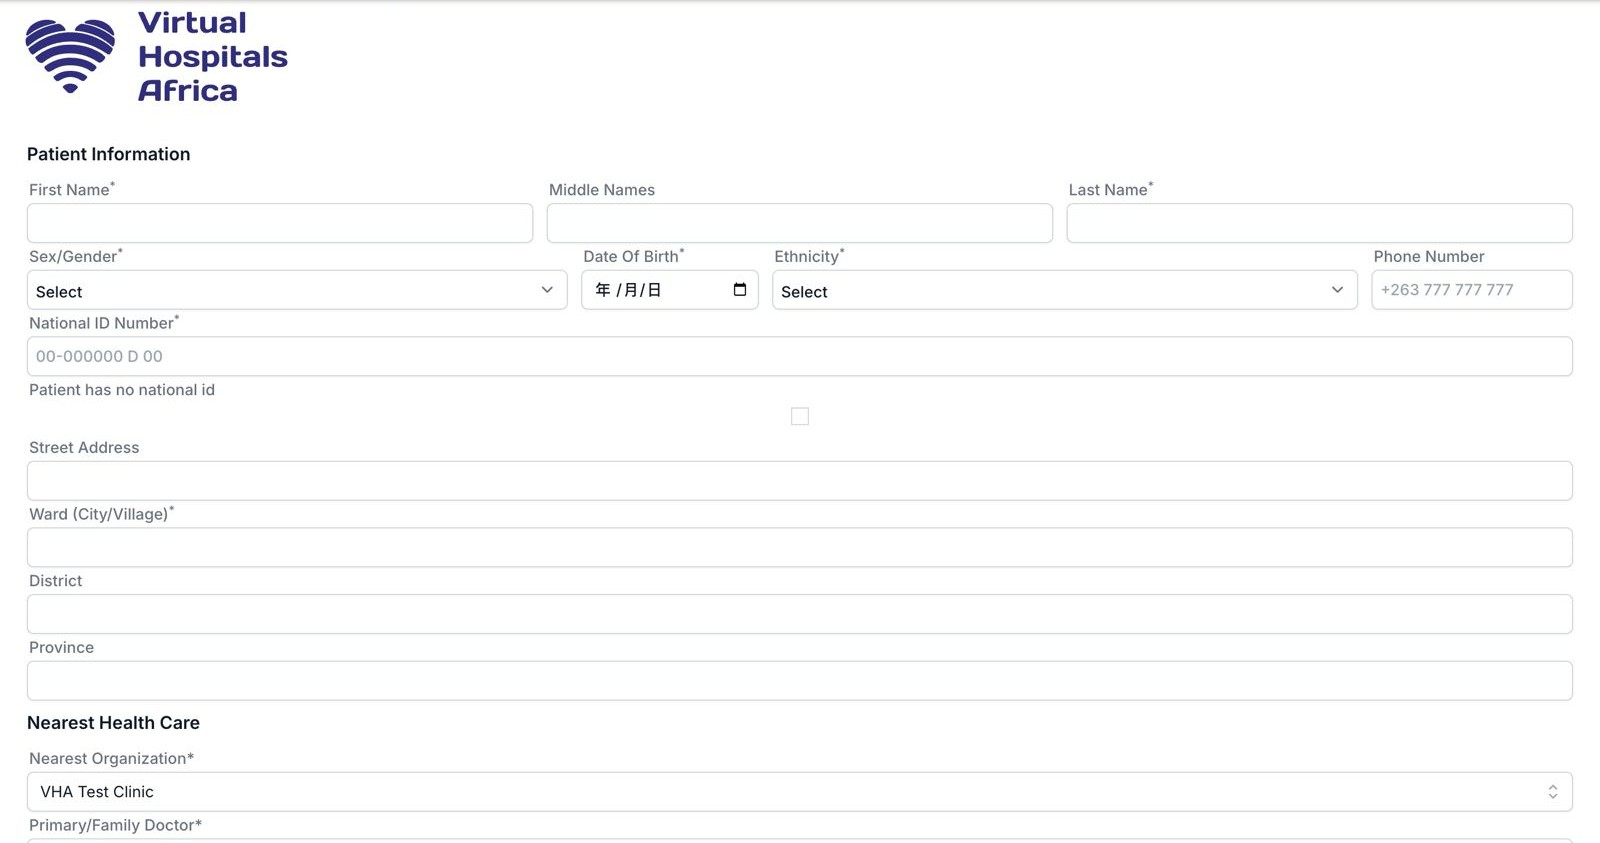
\includegraphics[width=\textwidth]{images/(VHA)-1.jpg}
        \caption{Patient Intake page – original version / user feedback context}
        \label{fig:design-1}
    \end{minipage}\hfill
    \begin{minipage}{0.47\textwidth}
        \centering
        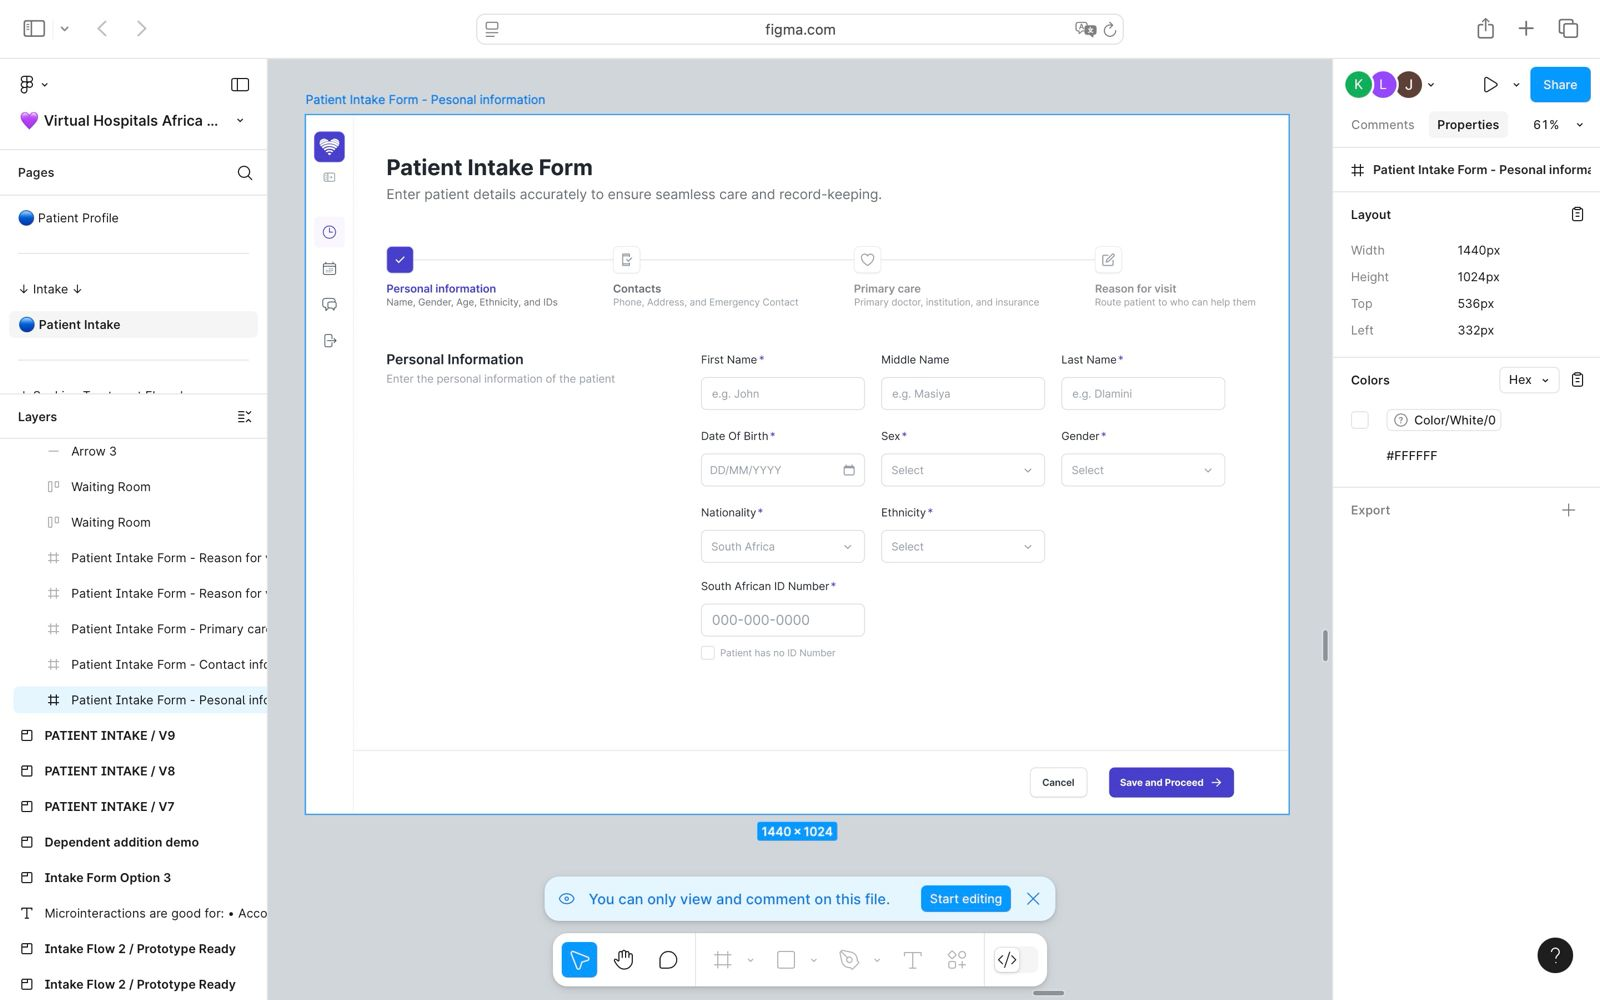
\includegraphics[width=\textwidth]{images/(VHA)-2.jpg}
        \caption{Second version multi-step form interface}
        \label{fig:design-2}
    \end{minipage}
\end{figure}
\begin{figure}[H]
    \centering
    \begin{minipage}{0.47\textwidth}
        \centering
        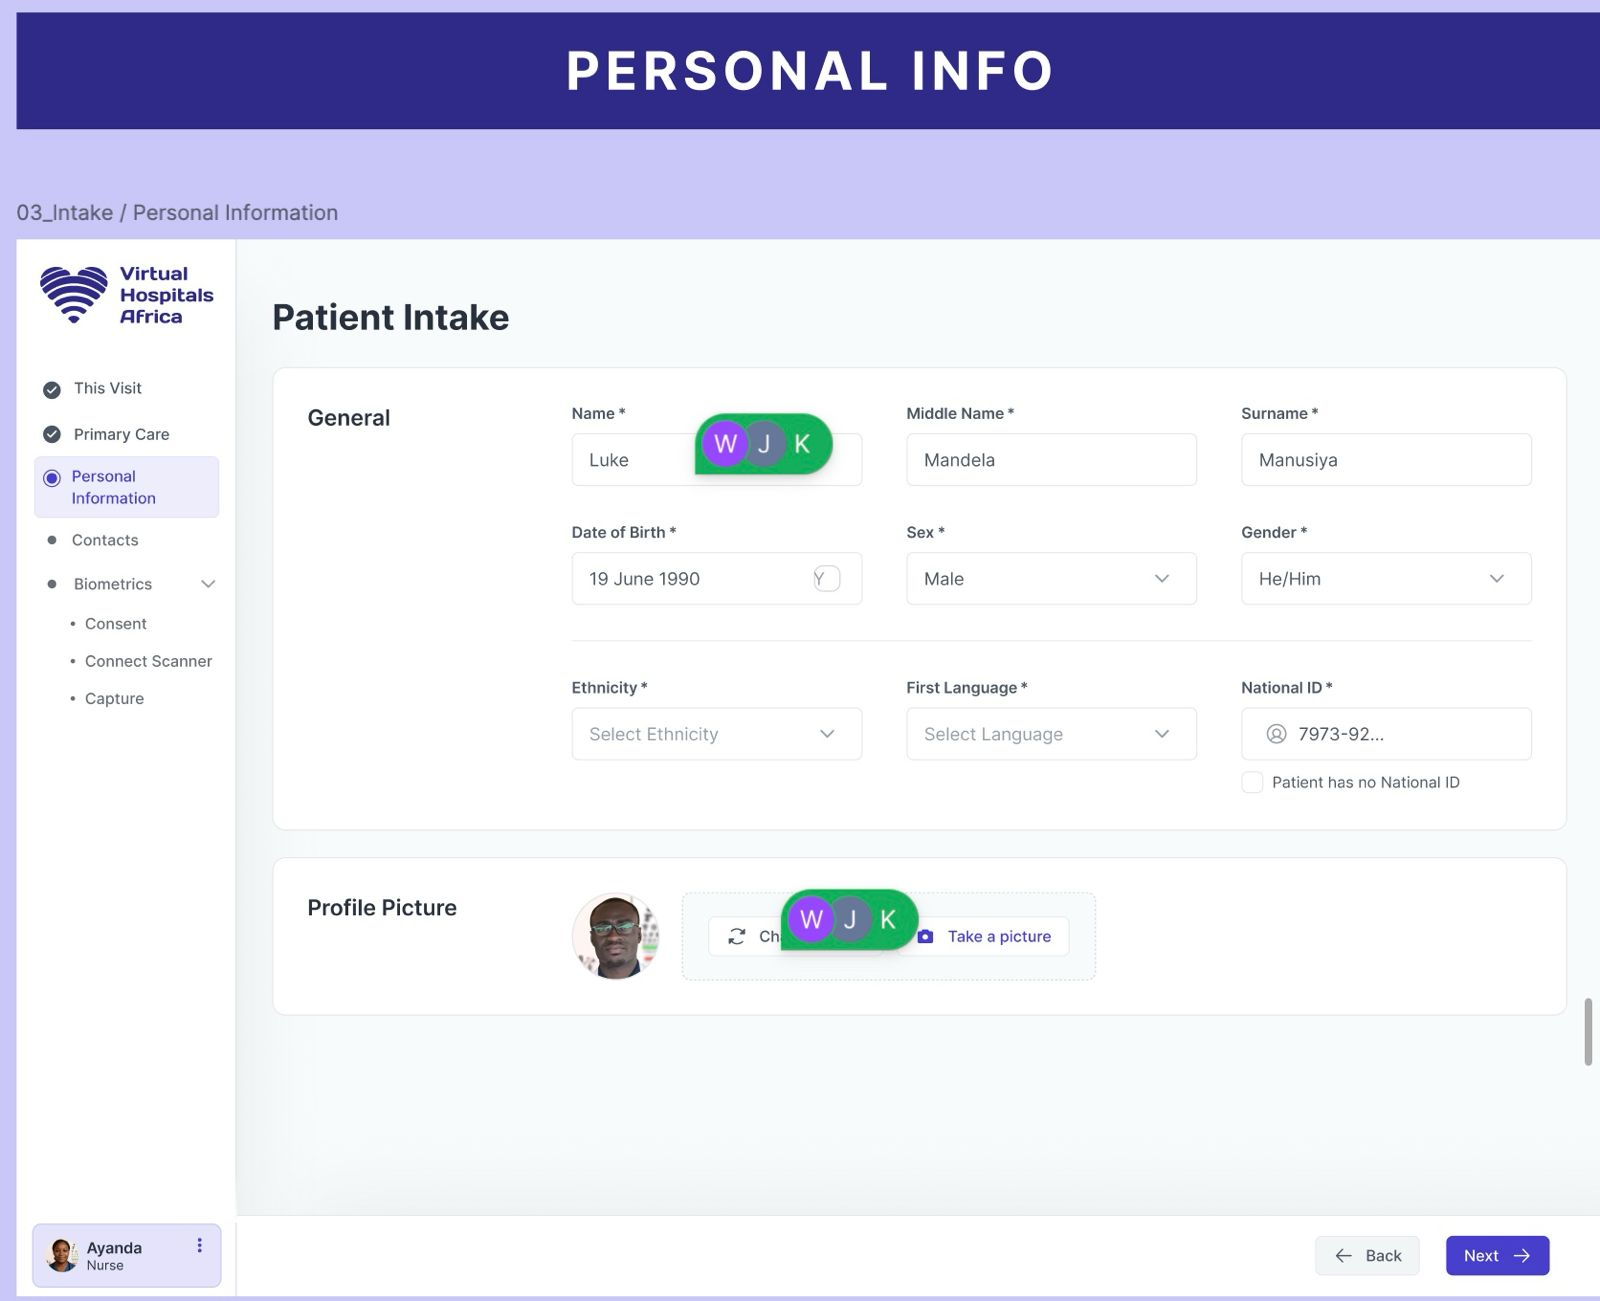
\includegraphics[width=\textwidth]{images/(VHA)-3.jpg}
        \caption{Third version with left-side navigation and unified buttons}
        \label{fig:design-3}
    \end{minipage}\hfill
    \begin{minipage}{0.47\textwidth}
        \centering
        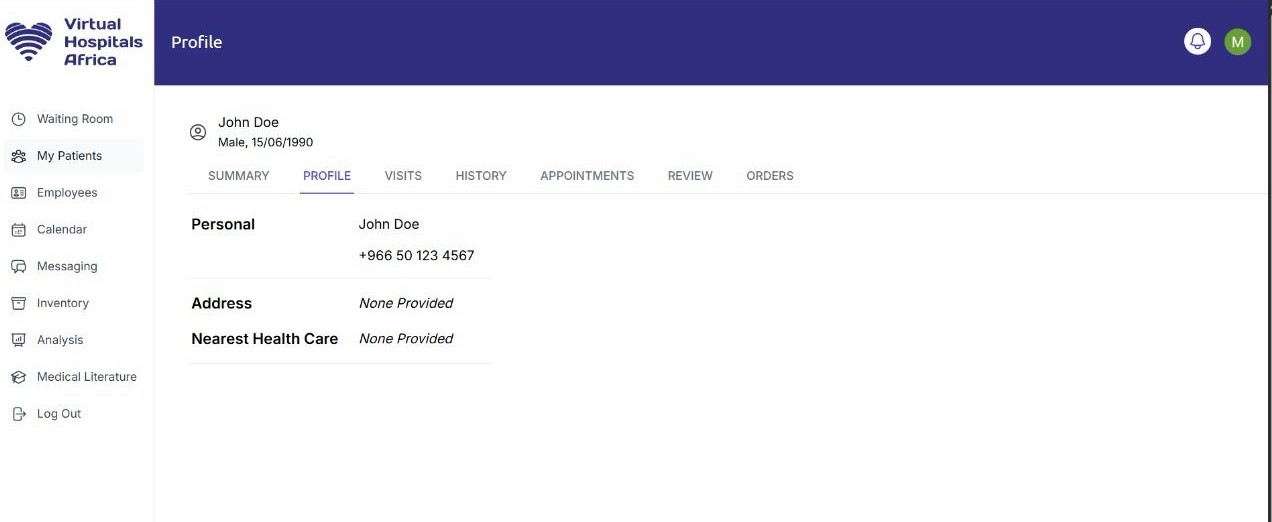
\includegraphics[width=\textwidth]{images/(VHA)-4.jpg}
        \caption{Patient profile page – issues in current interface}
        \label{fig:design-4}
    \end{minipage}
\end{figure}
\begin{figure}[H]
    \centering
    \begin{minipage}{0.47\textwidth}
        \centering
        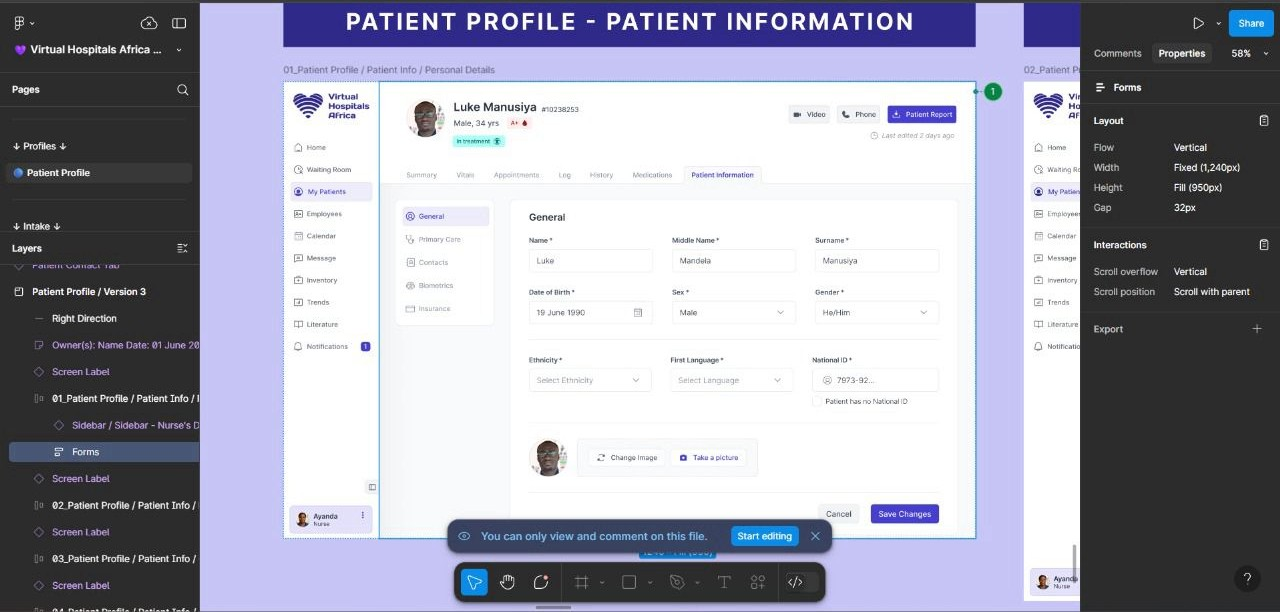
\includegraphics[width=\textwidth]{images/(VHA)-5.jpg}
        \caption{Redesigned patient profile with improved info card and modules}
        \label{fig:desbign-5}
    \end{minipage}\hfill
    \begin{minipage}{0.47\textwidth}
        \centering
        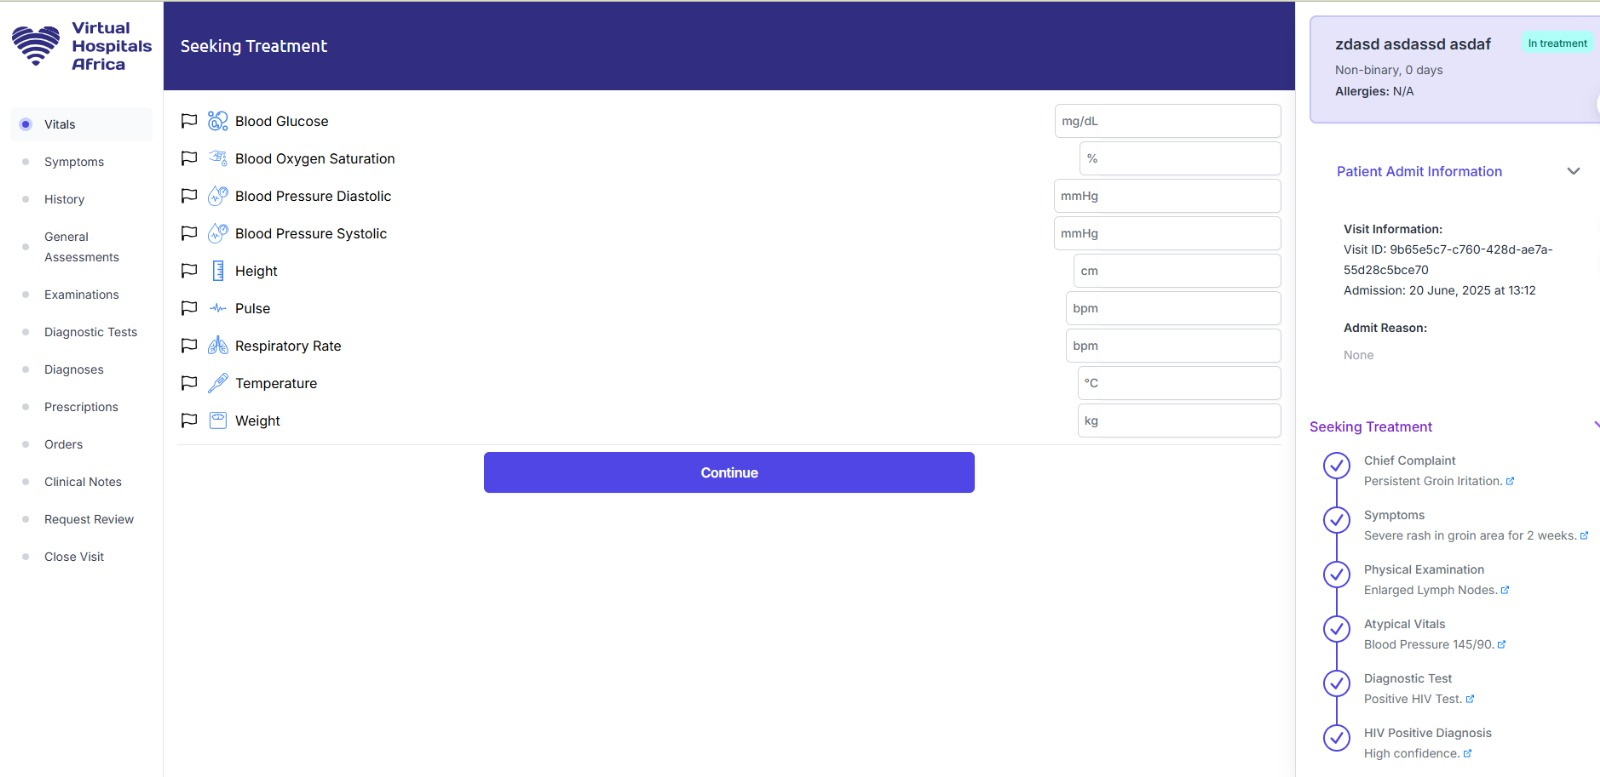
\includegraphics[width=\textwidth]{images/(VHA)-6.jpg}
        \caption{Vitals page – issues in original layout}
        \label{fig:design-6}
    \end{minipage}
\end{figure}

\subsection{Code Implementation - Patient Data Management}

Virtual Hospital Africa's goal is to implement a virtual hospital website with a fast user interface that is also maintainable and adaptable. Achieved by using type-safe frameworks, such as TypeScript and React, to ensure code quality and reduce runtime errors and the utility first approach with tailwind CSS.

\paragraph{TypeScript}\mbox{}

TypeScript is a superset of JavaScript which allows developers to catch errors at compile time rather than runtime, making it easier to maintain and refactor code. It provides static type checking, which helps in identifying any potential issues early in the development process. This is particularly useful for large codebases like Virtual Hospital Africa, where maintaining code quality and consistency is crucial. The codebase demonstrates type definitions for complex data structures, as shown in the patient management system components. TypeScript's type system provides significant advantages in large-scale application development by enabling early error detection and improved code maintainability (Bierman et al., 2014).

The implementation showcases strong type safety through interfaces and type definitions. For example, the \texttt{Measurements} definition in \texttt{type.ts} includes precise geographic positioning with \texttt{latitude: number} and \texttt{longitude: number} properties, along with optional \texttt{admit\_reasons?: string[]} arrays. The patient data structure demonstrates TypeScript's nullable type handling with properties like \texttt{age\_years?: Maybe<number> | string | null}, showcasing the framework's flexibility in handling uncertain data states.

The SQL integration in \texttt{patient.ts} demonstrates TypeScript's template literal types and generic constraints with complex database queries: \texttt{\detokenize{sql<string | null>`
\patient_age.age_years::text`.as('age_years')`}} and string interpolation for formatted patient data. This ensures type safety in SQL queries, preventing runtime errors and increasing code reliability.

Interface Segregation Principles (ISP) guide the API contracts and the component props  design. this makes sure that the components only recieve the necessary data they need to function. Generic types enable reusable components that work with different data types whilst maintaining type safety. The implementation includes comprehensive error handling with typed error objects and proper exception management, leveraging TypeScript's structural type system to ensure compile-time safety (Bierman et al., 2014).

\paragraph{Tailwind CSS}\mbox{}

Tailwind CSS is a utility-first CSS framework that allows developers to create custom designs without writing custom CSS. It provides a set of pre-defined classes that can be combined to build complex user interfaces. This approach promotes consistency and reusability across the code, making it easier to maintain and adapt the design as needed.
The implementation includes a custom configuration that defines design tokens, colour palettes, typography scales, and spacing systems for each project. The structure adds custom colours, fonts, and breakpoints to the default theme to meet the design needs. Customised utility classes manage unique designs and varying components  that go further than the built-in utilities. The solution uses Just-In-Time compilation for the best speed and decreased bundle sizes(Tailwind Labs, 2024). Component variations and responsive designs tools make certain that style remains consistent across varying screen sizes as well as devices. The approach to style highlights atomic CSS classes for rapid prototype development while retaining a design consistency employing a well-defined design system.

\paragraph{Component Architecture}\mbox{}

The \texttt{PatientDrawerV2} component in \texttt{DrawerV2.ts} shows a well-structured component architecture. This component demonstrates an organised approach to feature components, handling complex patient data presentation with the proper TypeScript interfaces.
The component accepts a comprehensive props interface that includes nested object types:

\begin{verbatim}
patient: {
  id: string
  name: string
  description: string | null
  avatar_url?: Maybe<string>
  date_of_birth?: string
  dob_formatted?: string | null
  gender?: Maybe<Gender>
  age?: number
  age_year?: number
  age_years?: Maybe<number> | string | null
  age_display?: Maybe<string>
  allergies?: string
  actions: {
    view: string
  }
}
\end{verbatim}

This demonstrates how nested data structures are managed with union types and other optional properties.
Layout components handle the overall application structure including headers, navigation, sidebars, and footer elements. These components provide consistent positioning and responsive behaviour across all application pages. UI components represent reusable interface elements such as buttons, forms, modals, and data display components. Feature components encapsulate specific business logic and user interactions related to particular application features. Page components serve as containers that compose multiple components to create complete user interfaces. This hierarchical approach enables efficient code reuse and simplified maintenance.

The \texttt{PatientDrawerV2} component demonstrates implementation patterns with comprehensive error handling and type safety. Research indicates that TypeScript adoption in frontend development significantly reduces runtime errors and improves code maintainability (Chen et al., 2019). The component includes customised utility functions such as \texttt{calcutaeAge()} and \texttt{formatAge()} which showcase input validation and error handling:
\begin{verbatim}
  export function calculateAge(dateOfBirth: string): number {
  if (!dateOfBirth) {
    return 0
  }

  const birthDate = new Date(dateOfBirth)

  if (isNaN(birthDate.getTime())) {
    console.log('Invalid birth date:', dateOfBirth)
    return 0
  }

  const today = new Date()
  let age = today.getFullYear() - birthDate.getFullYear()
  const monthDiff = today.getMonth() - birthDate.getMonth()
  if (monthDiff < 0 || monthDiff === 0 && today.getDate()
  < birthDate.getDate()) {
    age--
  }
  return age
}
\end{verbatim}
This function establishes null checking and type validation as well as error handling. Edge cases are handled by the age calculation logic and are provided fallback values to ensure the component remains functional even with invalid or incomplete data. The component also showcases union type handling in the age display logic, where multiple data sources are checked in priority order:
\begin{verbatim}
     Primary - patient.age_year
     Formatted display - patient.age_display
     Fallback numeric value - patient.age
   	 Calculated from patient.date_of_birth or patient.dob_formatted
\end{verbatim}
Higher-order components and render props enable component composition whilst maintaining type safety. Furthermore, this implementation uses generic constraints to ensure proper type inference in composed components. Context providers manage global state and shared functionality with typed context values.

The code further demonstrates complex error handling of medical data with type safety measures. in \texttt{family.tsx}, the execution shows data validation:
\begin{verbatim}
  const patient_id = ctx.state.patient.id
  const family = await patient_family.get(ctx.state.trx, { patient_id })
  assert(ctx.state.patient.age_years != null)
  const age_years = ctx.state.patient.age_years
  assert(typeof age_years === 'number' && age_years >= 0)
\end{verbatim}

This code runtime type assertions, database integrations, and data validation:

\textbf{Runtime Type Assertions:} Assert() statements are used to make sure the data conforms to the expected types and parameters at runtime, assisting in checking before compile time checking.

\textbf{Database Integrations:} The code integrates with the database to retieve family data for a patient, executed via \texttt{patient\_family.get()}. This method serves to maintain the type safety from the database layer to the user interface.

\textbf{Data Validation:} The validation \texttt{age\_years >= 0} demonstrates business logic validation, ensuring that healthcare data meets clinical requirements. The patient data structure supports multiple age representations, for instance \texttt{age, age\_year, age\_years, age\_display}, showing how the implementation handles legacy data\footnote{Data that is stored in a system which is outdated or now obsolete.} and multiple data sources whilst maintaining type safety. The code above also uses the state to be immutable\footnote{The value of the state cannot be changed once set.} e.g. \texttt{patient\_id}. State updates follow a clear data flow from parent to child components.Data fetching and caching optimise performance as well as user experience. The implementation includes loading states, error handling, and optimistic updates for API interactions. Custom hooks abstract data fetching logic and provide a consistent interface for the components to process API data.

\paragraph{Tailwind}\mbox{}

\texttt{PatientDrawerV2} component utilises utility classes for complex layouts and a responsive design:

\begin{verbatim}
  <div className='flex h-full flex-col overflow-y-scroll bg-white shadow-xl
  sticky right-0 min-w-[300px]'>
  <div className='bg-[hsla(245,75%,94%,1)] border-2
  border-solid border-[hsla(242,75%,87%,1)] rounded-lg p-4 m-4 shadow-sm'>
    <div className='flex justify-between items-start mb-2 leading-snug'>
\end{verbatim}

This implementation showcases these features:

\textbf{Responsive Layout:} Flexbox utilities such as \texttt{flex, flex-col,
justify-between, items-start}  are used for layout management and consistent spacing, and alignment across different screen sizes.

\textbf{Component State Styling:} Interactive elements like buttons and icons:
\begin{verbatim}
  <ChevronUpIcon
  className={`${
    open ? 'rotate-180 transform' : ''
  } h-5 w-5 text-gray-700`}
  strokeWidth={1}
/>
\end{verbatim}

\paragraph{Component Styling}\mbox{}

Component styling follows consistent patterns that promote maintainability and design coherence. Base component styles define default appearances and behaviours that can be extended through additional utility classes. Variant patterns handle different component states and appearances through prop-driven class application. The coding includes focus, hover and active states.

\paragraph{Performance Optimisation}\mbox{}


Tailwind's purge configuration removes unused CSS classes from the production build; significantly reducing bundle sizes. The includes purge patterns that scan all TypeScript and component files for used utility classes. Custom purge configurations handle dynamic class generation and conditional styling. The coding includes class concatenation utilities and conditional class application. Performance monitoring ensures optimal CSS bundle sizes and rendering performance.(Chen et al., 2019)

\paragraph{UX Implementation}\mbox{}

\texttt{PatientDrawerV2} shows user experience considerations. E.g. Date formatting is coded to be consistant withthe local setting.
\begin{verbatim}
  export function formatDate(date: string | Date): string {
  const Dates = new Date(date)

  if (isNaN(Dates.getTime())) {
    console.log('Invalid Date', date)
    return ''
  }

  return Dates.toLocaleDateString('en-GB', {
    year: 'numeric',
    month: 'short',
    day: '2-digit',
  })
}
\end{verbatim}

The code below is the date display logic in \texttt{PatientDrawerV2:}
\begin{verbatim}
  const day = date.toLocaleDateString('en-GB', { day: '2-digit' })
  const month = date.toLocaleDateString('en-GB', { month: 'long' })
  const year = date.toLocaleDateString('en-GB', { year: 'numeric' })
  const time = date.toLocaleTimeString('en-GB', { hour: 'numeric', minute:
  '2-digit' })
  return `${day} ${month}, ${year} at ${time}`
\end{verbatim}
